\chapter{Introducción específica} % Main chapter title

\label{Chapter2}

%----------------------------------------------------------------------------------------
%	SECTION 1
%----------------------------------------------------------------------------------------
En este capítulo se presentan las distintas tecnologías y metodologías disponibles para la implementación del prototipo de robot móvil. Se describen los dispositivos más significativos que permitieron alcanzar los requerimientos planteados.

\section{Diseño del prototipo}

El prototipo se diseñó para que una superficie plana sea irradiada con un dispositivo emisor de rayos ultravioletas de tipo C en forma teleoperada o haciendo un recorrido autónomo aleatorio.

Se utilizaron sensores infrarrojos y de contacto para evitar los obstáculos que puedan aparecer en el camino del robot. La información sensada se maneja en forma de valores booleanos, para simplificar el procesamiento, tanto en uso de memoria como en velocidad. 

La plataforma posee una placa de procesamiento central (EDU-CIAA) que recibe datos y una placa de control para el accionamiento de motores y/o dispositivos adicionales (como puede ser el encendido de LEDs UV-C germicidas). En la figura \ref{fig:blocks} se puede apreciar un diagrama con los principales bloques del dispositivo.


\begin{figure}[h]
	\centering
	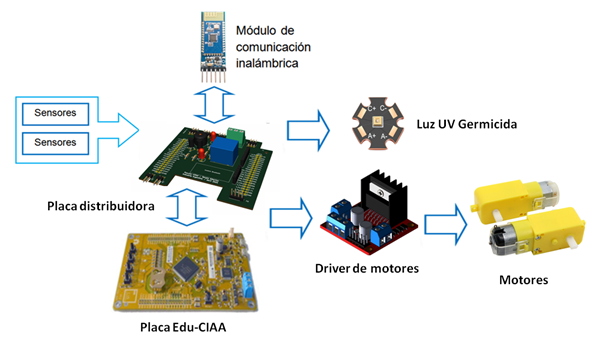
\includegraphics[width=\textwidth]{./Figures/blocks.png}
	\caption{Repressentación del robot para tareas de desinfección por UV-C.}
	\label{fig:blocks}
\end{figure}

El comportamiento general, en el modo autónomo, puede ser reconfigurado a través de una tabla disponible en una librería del programa, y generada por una aplicación en PC. Esto permite cambiar el comportamiento reactivo del robot, sin modificar la rutina principal de procesamiento, basada en máquina de estados.

Se construyó una estructura mecánica para contener las distintas partes de hardware electrónico, y poder ensayar el comportamiento de sensores y motores en su conjunto.

Si bien el prototipo robot contempla el recorrido sobre el piso, irradiando luz ultravioleta hacia abajo, no hay ningún impedimento para que los sensores se monten de forma que el robot pueda recorrer una superficie plana elevada (una mesa de trabajo, por ejemplo) sin caerse, o que el emisor de luz se encuentre en la parte lateral o superior (dado que es controlado en forma independiente).

No se plantean pruebas funcionales que demuestren que se han esterilizado microorganismos y virus al utilizar el dispositivo, dado que esto implicaría ensayos y estudios que exceden el equipamiento disponible y las aéreas de estudio de la especialización en sistemas embebidos.

El robot se alimenta con baterias recargables. No se  monitorea   ni se realiza la carga de las baterías y no se incluye cargador.
%----------------------------------------------------------------------------------------

\section{Módulos y dispositivos de hardware}
En esta sección se describen los módulos y dispositivos de hardware utilizados en el prototipo del robot desarrollado.

%----------------------------------------------------------------------------------------
\subsection{Placa de microprocesamiento}

Se decidió utilizar como hardware principal la placa de desarrollo EDU-CIAA-NXP \citep{EDUCIAA} para aprovechar la experiencia existente en la comunidad del posgrado.

En la figura \ref{fig:EDUCIAANXP} se observa una imagen de la EDU-CIAA-NXP, una versión de bajo costo de la CIAA-NXP, pensada para la enseñanza universitaria, terciaria y secundaria. 

\begin{figure}[htpb]
	\centering
	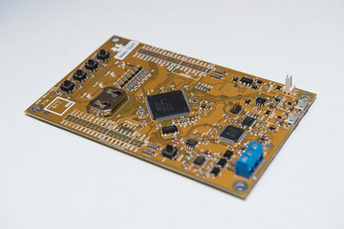
\includegraphics[width=\textwidth]{./Figures/EDUCIAANXP.jpg}
	\caption{Placa de desarrollo EDUCIAA-NXP\protect\footnotemark.}
	\label{fig:EDUCIAANXP}
\end{figure}
\footnotetext{Imagen tomada de \url{http://www.proyecto-ciaa.com.ar}}

\pagebreak

En la figura \ref{fig:Bloques} puede verse un diagrama en bloques general de la placa. 

\begin{figure}[htpb]
	\centering
	\includegraphics[width=9cm]{./Figures/Bloques.jpg}
	\caption{Diagrama en bloques de la EDUCIAA-NXP\protect\footnotemark.}
	\label{fig:Bloques}
\end{figure}
\footnotetext{Imagen tomada de \url{http://www.proyecto-ciaa.com.ar}}

El  microcontrolador utilizado por la EDU-CIAA es el LPC4337 (dual core ARM Cortex-M4F y Cortex-M0). Los recursos más significativos que se utilizaron de la placa fueron: 


\begin{itemize}
	\item GPIO (General Purpose Input/Output, Entrada/Salida de Propósito General)
	\item PWM (Pulse Width Modulation, modulación por ancho de pulso).
	\item UART (Universal Asynchronous Receiver-Transmitter, Transmisor-Receptor Asíncrono Universal).
	\item Temporizadores.
\end{itemize}

Para el accionamiento de los motores se utilizó modulación por ancho de pulsos (PWM, por su sigla en inglés). La placa EDU-CIAA posee un solo modulo PWM con 11 salidas asociadas. Todas las salidas PWM comparten la misma frecuencia, aunque puede asignarse un valor de ciclo de actividad en forma independiente.

%\begin{itemize}
%	\item PWM0:  GPIO\_2.
%	\item PWM1:  GPIO\_8.
%	\item PWM2:  T\_FIL1.
%	\item PWM3:  T\_FIL2.
%	\item PWM4:  T\_FIL3.
%	\item PWM5:  T\_COL0.
%	\item PWM6:  T\_COL1.
%	\item PWM7:  T\_COL2.
%	\item PWM8:  LCD\_1.
%	\item PWM9:  LCD\_2.		
%	\item PWM10: LCD\_3.				
%\end{itemize}
%
%Se utilizaron las líneas de T\_FIL3: PWM4 y T\_COL1: PWM6 para el control de los motores.


%----------------------------------------------------------------------------------------
\subsection{Motores}

El robot es impulsado por dos motores de corriente continua con reducción mecánica.

Para la selección de los motores se tuvieron en cuenta las características del prototipo a desarrollar. 
Las opciones típicas para este tipo de robot son los motores de corriente continua, los motores paso a paso y los servomotores \citep{servo}. 


En la tabla \ref{tab:comparacion} se listan ventajas y desventajas de estos tipos de motor.

 
\begin{table}[htpb]
\centering
\caption[comparacion]{Comparación de características según tipo de motor.}


\begin{tabular}{llll}
\hline
            & Motor de CC                                                                              & Motor paso a paso                                                                                                                                 & Servomotor                                                                                                                       \\ \hline
Ventajas    & \begin{tabular}[c]{@{}l@{}}Alta velocidad\\ y torque.\\ Fácil de controlar.\end{tabular} & \begin{tabular}[c]{@{}l@{}}Control de \\ posición sin \\ realimentación.\\ Precisión en \\ el control de \\ posición y \\ velocidad.\end{tabular} & \begin{tabular}[c]{@{}l@{}}Alta precisión \\ en control de \\ posición y \\ velocidad. \\ Circuito \\ realimentado.\end{tabular} \\ \hline
Desventajas & \begin{tabular}[c]{@{}l@{}}Requiere \\ reducción \\ mecánica.\end{tabular}               & \begin{tabular}[c]{@{}l@{}}Requiere \\ controlador.\\ Baja potencia.\end{tabular}                                                                 & \begin{tabular}[c]{@{}l@{}}Limitación\\ del recorrido. \\ Costoso.\end{tabular}                                                  \\ \hline
\end{tabular}
\label{tab:comparacion}
\end{table}

Los motores de corriente continua pueden alcanzar altas velocidades y un alto torque. Son fáciles de controlar, pero requieren de reducciones mecánicas cuando la velocidad de operación es baja.
Los motores paso a paso presentan precisión en sus movimientos sin requerir de realimentación,  pero exigen mayor electrónica para su control. Son muy efectivos para realizar desplazamientos cortos y precisos. Los servomotores  tienen un desplazamiento angular limitado y presentan gran precisión en movimientos cortos. Su principal  desventaja radica en el costo relativamente alto.

Se seleccionaron motores de corriente continua con caja reductora debido a que ofrecen las prestaciones suficientes para este tipo de robot, sin requerir de controladores (de hardware o software) adicionales \citep{motorcc}. 
En la figura \ref{fig:motorreductor} se puede ver una imagen del motor utilizado.

\begin{figure}[h]
	\centering
	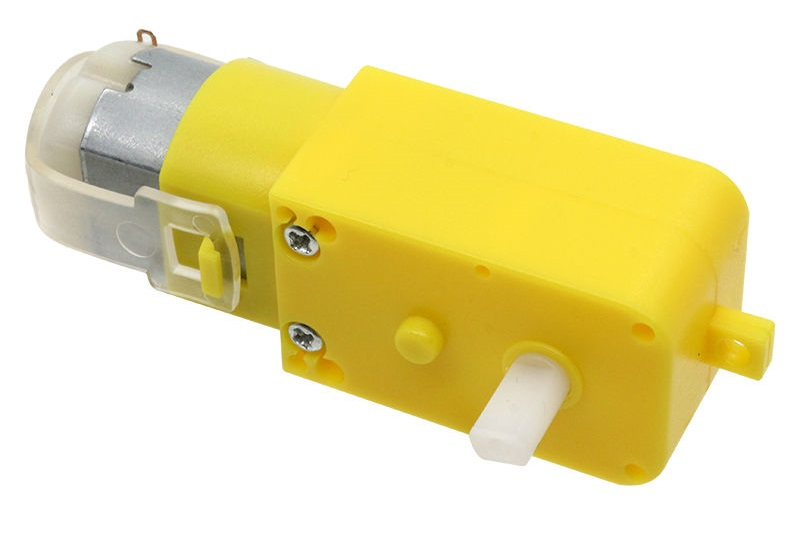
\includegraphics[width=7cm]{./Figures/Motorreductor.jpg}
	\caption{Imagen del motor utilizado\protect\footnotemark.}
	\label{fig:motorreductor}
\end{figure}
\footnotetext{Imagen tomada de \url{https://robots-argentina.com.ar/}}

Los motores elegidos cuentan con una caja de reducción (48:1) acoplada al eje del motor eléctrico, para lograr la disminución de velocidad, y un eje lateral que permite reducir espacio al utilizarlos en una configuración diferencial. La tensión nominal de trabajo va de los  3 a 6 V. Este modelo de motorreductor es ampliamente difundido en el mercado de componentes para robótica didáctica, por lo que es de fácil adquisición y bajo costo. 

En la tabla \ref{tab:caracteristicas} se referencian las principales características de los motores, según su tensión nominal de alimentación. 

\begin{table}[htpb]
\centering
\caption[características]{Características de los motores.}
\begin{tabular}{lccc}
                    & 3V DC       & 5V DC       & 6V DC      \\ \hline
Reducción           & \multicolumn{3}{c}{48:1}               \\
Velocidad sin carga & 125 RPM     & 200 RPM     & 230 RPM    \\
Velocidad con carga & 95 RPM      & 152 RPM     & 175 RPM    \\
Torque              & 0,8 kg.cm   & 1 kg.cm     & 1,1 kg.cm  \\
Corriente           & 110-130 mA  & 120-140 mA  & 130-150 mA \\
Dimensiones         & \multicolumn{3}{c}{70mm x 22mm x 18mm} \\
Peso                & \multicolumn{3}{c}{50g}                \\
Ruido               & \multicolumn{3}{c}{\textless{}65dB} 		\\  \hline
\end{tabular}
\label{tab:caracteristicas}
\end{table}


%En la figura \ref{fig:planomoto} se pueden observar las dimensiones del motor utilizado.
%
%%
%\pagebreak
%
%\begin{figure}[h]
%	\centering
%	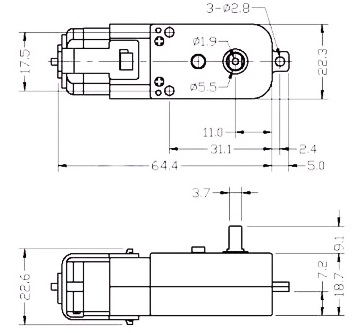
\includegraphics[width=9cm]{./Figures/planomoto.jpg}
%	\caption{Dimensiones del motor utilizado\protect\footnotemark.}
%	\label{fig:planomoto}
%\end{figure}
%\footnotetext{Imagen tomada de \url{https://robots-argentina.com.ar/}}





\subsection{Driver de motores}
Para el accionamiento de los motores se decidió utilizar un módulo basado en el circuito integrado L298N \citep{L298}. Este módulo tiene una configuración de doble puente H que permite  controlar dos motores de corriente continua de manera simultánea e independiente. 
El módulo ofrece conectores de entrada y salida para el puente integrado, un regulador LM78M05 interno que suministra 5V para la lógica de control, y los  los diodos de protección de contracorriente en las salidas \citep{Driver}.

En la figura \ref{fig:Driver} se puede observar una imagen de la placa y sus conectores. Sus características principales son:

\begin{itemize}
	\item Tensión mínima: 5 V.
	\item Tensión máxima: 35 V.
	\item Corriente máxima: 2 A.
	\item Tensión de nivel lógico: 5 V.
	\item Potencia máxima 25 W.
	\item Medidas: 43 x 43 x 24 mm.
\end{itemize}
%\pagebreak

\begin{figure}[h]
	\centering
	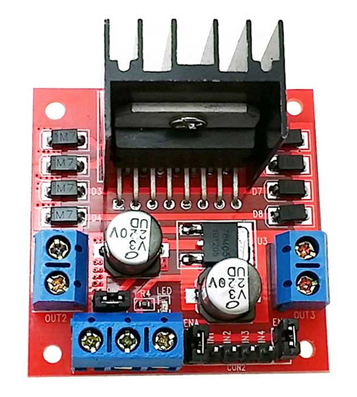
\includegraphics[width=6cm]{./Figures/L298N.png}
	\caption{Driver de motores\protect\footnotemark.}
	\label{fig:Driver}
\end{figure}
\footnotetext{Imagen tomada de \url{http://robots-argentina.com.ar}}


La placa tiene la opción de habilitar o no el regulador LM7805 integrado para alimentar la parte lógica. En la figura \ref{fig:Esquema} se observa el diagrama esquemático del módulo.


\begin{figure}[h]
	\centering
	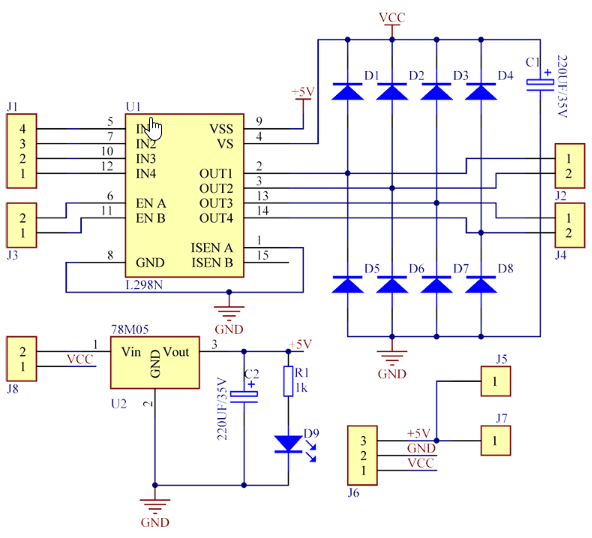
\includegraphics[width=11cm]{./Figures/Modulo.png}
	\caption{Diagrama esquemático del módulo\protect\footnotemark.}
	\label{fig:Esquema}
\end{figure}
\footnotetext{Imagen tomada de \url{http://robots-argentina.com.ar}}


%----------------------------------------------------------------------------------------

\subsection{Módulo sensor de infrarrojos}

Se utilizaron dos módulos sensores de proximidad por infrarrojos IR FC-51 \citep{IR} para la detección de obstáculos por parte del robot. Estos módulos están compuestos por  un emisor de luz infrarroja (IR)  y un receptor que detecta su reflejo en  las superficies contra las que se enfrenta, de modo que presentan una señal en  presencia de cualquier obstáculo en su parte frontal. 

El sensor presenta una respuesta estable incluso con luz ambiente o en completa oscuridad. En la figura \ref{fig:moduloIR} se observa una imagen del sensor de infrarrojos.

\begin{figure}[h]
	\centering
	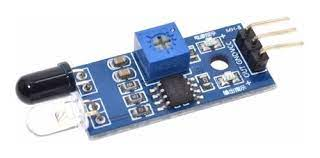
\includegraphics[width=8cm]{./Figures/moduloIR.jpg}
	\caption{Módulo sensor de infrarrojos \protect\footnotemark.}
	\label{fig:moduloIR}
\end{figure}
\footnotetext{Imagen tomada de \url{http://robots-argentina.com.ar}}

Las características del módulo son:
\begin{itemize}
	\item Ángulo de cobertura: 35°.
	\item Tensión de funcionamiento: 3 V – 6 V.
	\item Rango de detección: 2 cm – 30 cm (ajustable con el potenciómetro).
	\item Tamaño: 4,5 cm x 1,4 cm x 0,7 cm. 
	\item Discriminación: la salida toma nivel lógico bajo cuando se detecta un obstáculo (reflexión).
\end{itemize}

El circuito electrónico del módulo se basa en un amplificador operacional integrados LM339 utilizado como comparador entre la señal obtenida del receptor infrarrojo y un nivel de tensión determinado por un potenciómetro, lo cual permite ajustar el rango de distancia de la detección de obstáculo. En la figura \ref{fig:IRschem} se muestra el circuito esquemático del sensor de infrarrojos

\begin{figure}[h]
	\centering
	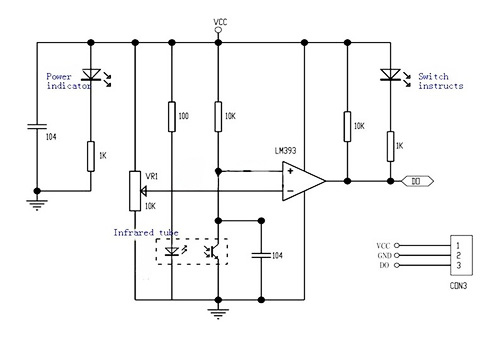
\includegraphics[width=14cm]{./Figures/IRschem.jpg}
	\caption{Diagrama esquemático del módulo sensor de infrarrojos\protect\footnotemark.}
	\label{fig:IRschem}
\end{figure}
\footnotetext{Imagen tomada de \url{http://robots-argentina.com.ar}}
%\pagebreak




%----------------------------------------------------------------------------------------
\subsection{Módulo detector pasivo de infrarrojos}

Se utilizó un módulo detector pasivo de infrarrojos (PIR) para poder sensar movimientos alrededor del robot cuando está encendido el módulo UV-C y desactivarlo para evitar la irradiación sobre personas o animales que se acerquen al robot. 
Los detectores PIR captan la variación de las radiaciones infrarrojas del medio ambiente que los rodea y de esa manera reaccionan ante fuentes de energía tales como el calor del cuerpo humano o de animales. Es llamado pasivo debido a que no emite radiaciones, sino que las recibe. Su funcionamiento se basa en un sensor piroeléctrico que es un componente electrónico diseñado para detectar cambios en la radiación infrarroja recibida. 

Se utilizó un módulo PIR HC-SR501 \citep{PIR} que cuenta con dos potenciómetros para regular la sensibilidad y el tiempo de duración del pulso. Las principales características son:

\begin{itemize}
	\item Tensión de operación: 4,5 V - 20 V.
	\item Corriente en reposo: <50 uA.
	\item Rango de detección: 3 a 7 metros (ajustable).
	\item Tiempo de retardo: 5 - 200 Seg (puede ser ajustado).
	\item Angulo de detección: <100º (cono).
	\item Tamaño: 3,2 cm x 2,4 cm x 1,8 cm.
\end{itemize}

En la figura \ref{fig:pir} se puede ver una imagen del módulo PIR HC-SR501 utilizado.

\begin{figure}[h]
	\centering
	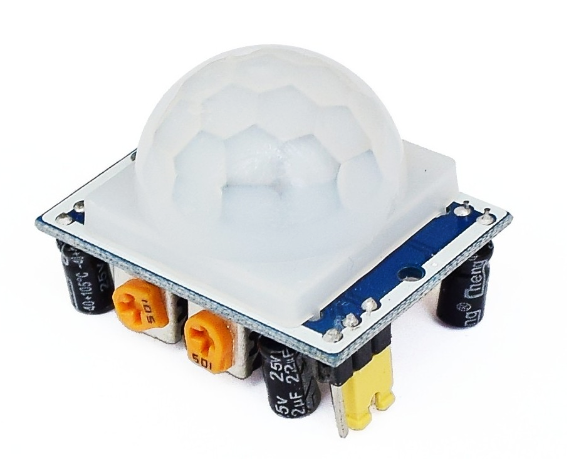
\includegraphics[width=8cm]{./Figures/pir.PNG}
	\caption{Módulo PIR HC-SR501\protect\footnotemark.}
	\label{fig:pir}
\end{figure}
\footnotetext{Imagen tomada de \url{https://naylampmechatronics.com/}}


%----------------------------------------------------------------------------------------
\subsection{Buzzer o transductor electroacústico}

Se utilizó un buzzer o transductor electroacústico para la señalización sonora sobre el estado de operación del robot. El transductor produce un tono audible, generado por un diafragma piezoeléctrico. 
El buzzer seleccionado es de tipo Activo, es decir que posee un oscilador incorporado al dispositivo. 
Sus características técnicas son:

\begin{itemize}
	\item Tensión de operación: 3,3 V ~ 5 V.
	\item Corriente de operación: <25 mA.
	\item Salida de sonido min a 10 cm: 85 dB.
	\item Frecuencia: 3,1 kHz. 	
	\item Diámetro: 12 mm.
	\item Altura: 7,5 mm.
	\item Longitud: 7,5 mm.	
\end{itemize}


En la figura \ref{fig:buzzer2} se observa imagen del transductor electroacústico utilizado.

\begin{figure}[h]
	\centering
	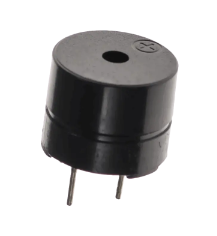
\includegraphics[width=3cm]{./Figures/buzzer2.PNG}
	\caption{Imagen del buzzer seleccionado\protect\footnotemark.}
	\label{fig:buzzer2}
\end{figure}
\footnotetext{Imagen tomada de \url{https://sumador.com/products/buzzer-activo-5v-12x9-5mm}}
%%

%----------------------------------------------------------------------------------------
\subsection{LED ultravioleta }

El robot cuenta con un relé para la activación del módulo UV-C. De esta manera el dispositivo emisor de luz ultravioleta puede tener alimentación independiente y hasta intercambiarse por otro de distintas prestaciones.
Para el desarrollo del prototipo se optó por un emisor LED de alta potencia, alimentado con la misma batería del robot, siendo que   son más compactos y resistentes a los golpes que las lámparas ultravioleta halógenas y emiten menos radiación de calor, por lo que pueden montarse más fácilmente sin tener que contar con disipadores adicionales. 
Los LEDs UV-C presentan un ángulo de apertura que oscila alrededor de los 120 grados con lo que es más fácil dirigir toda la potencia de radiación UV a una superficie específica.
Se utilizó un LED de alta potencia, germicida, tipo SMD3535, para el módulo de desinfección. Sus características técnicas son las siguientes:

\begin{itemize}
	\item Tipo de LED:		SMD3535.
	\item Color:		Ultravioleta UVC .
	\item Potencia:		1 W.
	\item Corriente		120 mA.	
	\item Tensión de Entrada:	5 a 8 VDC.
	\item Flujo Radiante:	7 - 12 mW.
	\item Longitud de Onda:	280 nm.
	\item Apertura del Haz:	140 grados.	
	\item Vida útil:	30000 horas.	
	\item Diámetro:		6,5 mm.	
	\item Largo:		15,5 mm.	
	\item Ancho:		8 mm.		
	\item Alto:			5,2 mm.		
	\item Peso: 		120 g.		
\end{itemize}


En la figura \ref{fig:leduvc} se observa imagen del LED UVC Germicida.

\begin{figure}[h]
	\centering
	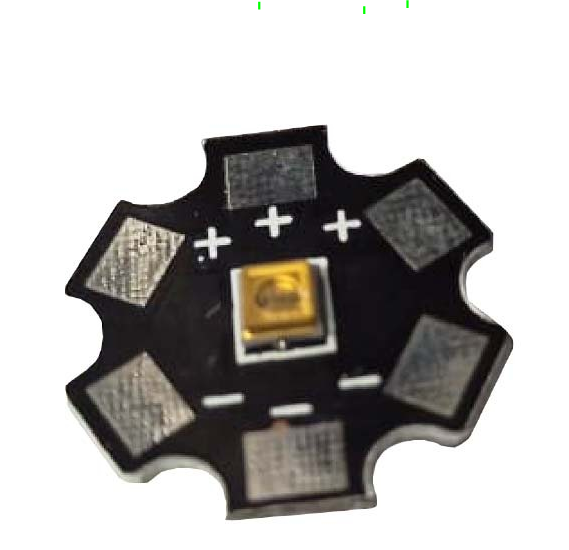
\includegraphics[width=4cm]{./Figures/leduvc.PNG}
	\caption{imagen del LED UVC Germicida seleccionado\protect\footnotemark.}
	\label{fig:leduvc}
\end{figure}
\footnotetext{Imagen tomada de \url{https://www.dled.com.ar}}
%%

%----------------------------------------------------------------------------------------
\subsection{Módulo de comunicaciones Bluetooth}

%Siendo que el prototipo robot se diseñó para su uso en ambientes interiores, la distancia del enlace no requiere un valor mayor al de algunos metros. Además la tasa de transferencia de datos no es alta, por lo que el ancho de banda no constituye un parámetro limitante. 

Se utilizó el módulo Bluetooth HC-05 para la comunicación con el robot \citep{HC05}. El mismo ya había sido utilizado en  prácticas de la asignatura "protocolos de comunicación en sistemas embebidos”.
El módulo permite realizar un enlace digital con un alcance de 10 m aproximadamente y no requiere antena externa ya que se encuentra integrada en el PCB. La velocidad máxima de transmisión asincrónica es de 2 Mbps y soporta modo master y modo slave.

En la figura \ref{fig:moduloHC05} se observa el módulo HC-05.


\begin{figure}[h]
	\centering
	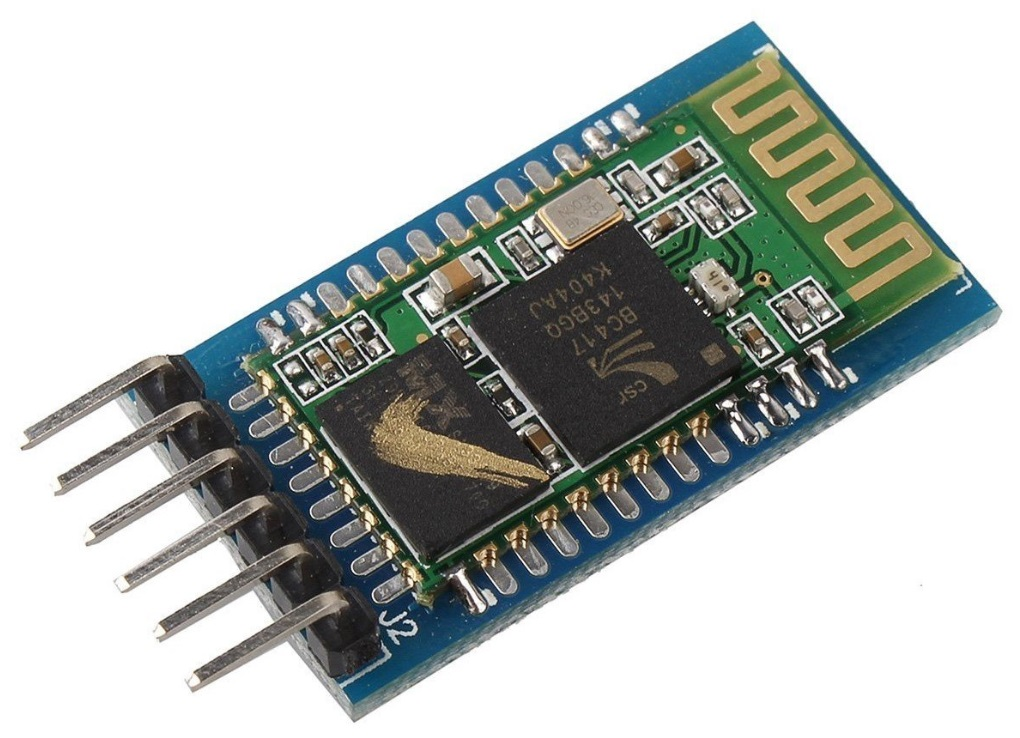
\includegraphics[width=6cm]{./Figures/HC05.jpeg}
	\caption{Módulo Bluetooth HC-05\protect\footnotemark.}
	\label{fig:moduloHC05}
\end{figure}
\footnotetext{Imagen tomada de \url{https://www.todomicro.com.ar/arduino/222-modulo-bluetooth-hc05}}


Las características del módulo son:
\begin{itemize}
	\item Tensión de operación: 3,6 V - 6 V DC.
	\item Consumo corriente: 50 mA.
	\item Bluetooth: V2.0+EDR.
	\item Frecuencia: banda ISM 2,4 GHz.
	\item Modulación: GFSK (Gaussian Frequency Shift Keying).
	\item Potencia de transmisión: 4 dBm, Class 2.
	\item Sensibilidad: -84 dBm a 0.1\% BER.
	\item Alcance 10 m.
	\item Tamaño: 3,7 cm x 1,6 cm.
\end{itemize}

El módulo HC-05 está configurado de fábrica como dispositivo esclavo (slave), pero se puede cambiar para que trabaje como maestro (master). También es posible modificar el nombre, código de vinculación, velocidad y otros parámetros mediante comandos AT \citep{HC05}. 

%\pagebreak


\subsection{Baterías}

En función del consumo y la intensión de no dedicar mayor espacio a las celdas de alimentación, se emplearon dos baterías de Ion-litio tipo 18650. La capacidad de estas baterías varía de un modelo a otro pero suelen estar comprendidas entre los 2100 y los 4000 mAh, y  permiten ser recargadas con una media de entre 600 a 1000 veces sin que se estropeen ni pierdan efectividad \citep{18650}. Su tensión nominal es de 3,7V, e incluso puede alcanzar los 4,2V en vacío.

Las baterías van conectadas en serie para lograr una tensión de 7,4 V, acorde a la alimentación de los motores, y con un margen superior necesario para el correcto funcionamiento del regulador de tensión de 5 V del módulo de accionamiento de motores. 
Las baterías se insertaron en un portapilas comercial. En la figura \ref{fig:portapila} se muestra las dos baterías 18650 ya instaladas en su portapila.


\begin{figure}[h]
	\centering
	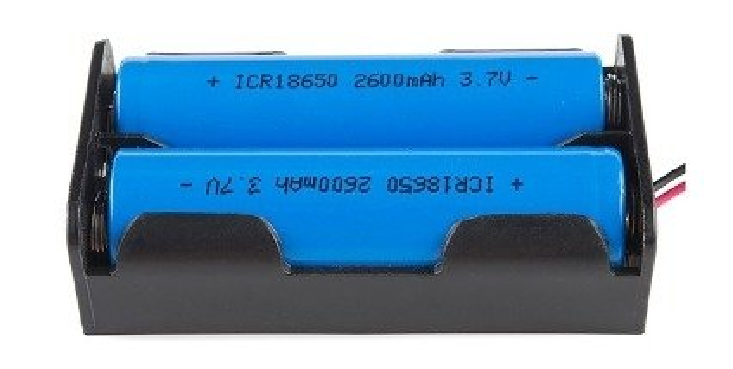
\includegraphics[width=10cm]{./Figures/portapilas.PNG}
	\caption{Baterías 18650 en su portapila .}
	\label{fig:portapila}
\end{figure}



%\section{Módulos de software}
%%En esta sección se describen los módulos de software utilizados.
%
%Se utilizaron módulos de software de la biblioteca sAPI \citep{sapi} del firmware de la EDU-CIAA versión 3 para acceder de manera simple a los diferentes periféricos.

\section{Entorno gráfico para el desarrollo de la aplicación móvil}

Para el desarrollo de la aplicación móvil se utilizó MIT App Inventor. Se trata de un entorno gráfico de programación desarrollado por Google Lab y administrado por el Instituto Tecnológico de Massachusett (MIT)\citep{MIT}, que utiliza un lenguaje visual basado en bloques el cual permite en forma sencilla programar aplicaciones totalmente funcionales para dispositivos que utilicen el sistema operativo Android \citep{android}.
La herramienta es de distribución gratuita y aunque las aplicaciones desarrolladas  en este entorno no alcanzan una gran complejidad, es posible cubrir con ellas un gran número de necesidades básicas en un dispositivo móvil.

El entorno cuenta con un módulo de diseño denominado App Inventor Designer con el que se desarrolla el contenido y la apariencia de la aplicación. En la figura \ref{fig:mitappdes} se observa la pantalla de diseño.

\begin{figure}[h]
	\centering
	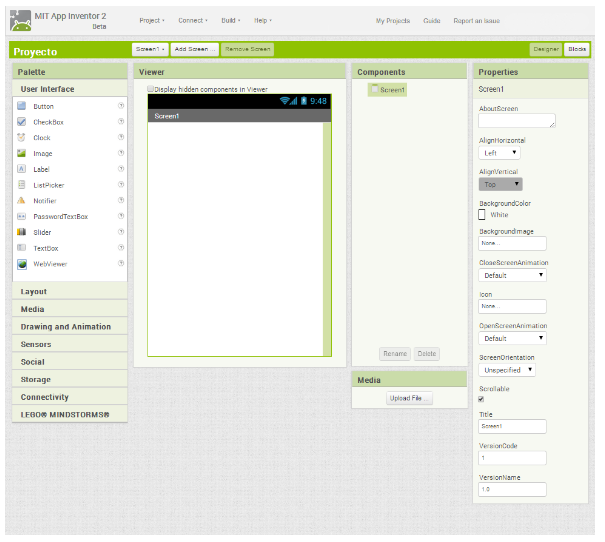
\includegraphics[width=12cm]{./Figures/appinventordesigner.PNG}
	\caption{Pantalla del módulo App Inventor Designer\protect\footnotemark..}
	\label{fig:mitappdes}
\end{figure}
\footnotetext{Imagen tomada de \url{https://diocesanos.es/blogs/equipotic/2015/05/16/mit-app-inventor-programando-aplicaciones-para-android/}}


Para la programación de la aplicación MIT App Inventor cuenta con un módulo editor de bloques denominado App Inventor Blocks Editor, que permite la programación en forma visual del comportamiento de los distintos  componentes de la aplicación, al ensamblar los bloques como piezas de un esquema. En la figura \ref{fig:mitappblock} se observa cómo se conforma el programa usando el editor de bloques.


\begin{figure}[h]
	\centering
	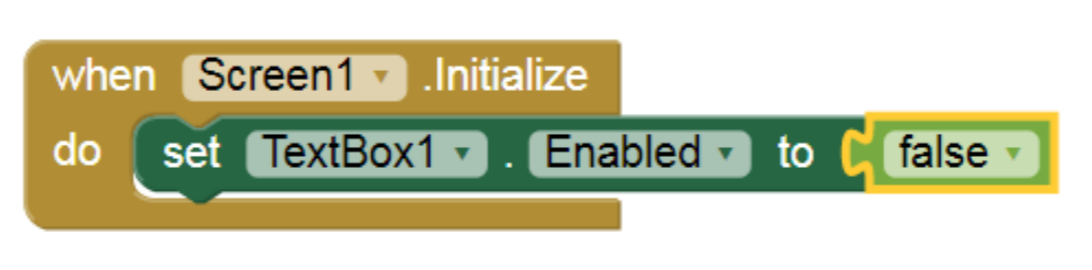
\includegraphics[width=8cm]{./Figures/mitblock.PNG}
	\caption{Ejemplo de programación en bloques usando App Inventor Blocks Editor.\protect\footnotemark..}
	\label{fig:mitappblock}
\end{figure}
\footnotetext{Imagen tomada de \url{https://docs.google.com/presentation/d/1jKjbLS9AFnHildJjZ8o4Jd7ou_ejwAmtdI0GGi0Jg48}}


Como aspecto positivo del uso de MIT App Inventor cabe resaltar que se trata de un software gratuito y de fácil configuración, al que se puede acceder desde cualquier computadora sin necesidad de instalarlo
Las limitaciones principales del uso de MIT App Inventor radican en que solo permite desarrollos para la plataforma Android, y que no se puede acceder a la interfaz de desarrollo (IDE) sin conexión a internet.

%\pagebreak

%%----------------------------------------------------------------------------------------
%%	SECTION 2
%%-----------------------------------------------------------------
%\section{Requerimientos}
%
%En esta sección se enumeran los requerimientos planteados en la planificación inicial del proyecto.  Los  requerimientos se han dividido en funcionales y no funcionales.
%
%\label{sec:requerimientos}
%
%\begin{enumerate}
%\item Requerimientos funcionales
%	\begin{enumerate}
%	\item Capacidad de locomoción.  El robot debe ser capaz de desplazarse por medio de ruedas motorizadas, a través de superficies planas.
%	\item Capacidad de percepción. El robot debe ser capaz de detectar y obtener información del medio. 
%	\item Capacidad de comunicación inalámbrica. El robot sebe ser capaz de establecer una comunicación  por medio de un módulo Bluetooth, con una aplicación android en un celular o tablet.
%	\item El robot deberá funcionar con alimentación a batería recargable.
%	\item El proyecto debe ser extensible a una posible herramienta de enseñanza e investigación.
%
%	\end{enumerate}
%\item Requerimientos no funcionales
%	\begin{enumerate}
%	\item El robot no debe emitir luz UV-C cuando detecte movimiento a su alrededor, para no producir daños a la salud de personas o animales con los que interactue.
%	\item El diseño del robot debe respetar regulaciones en cuanto a radiación en el espectro ultravioleta.
%	\item Se utilizarán componentes electrónicos disponibles comercialmente en Argentina.
%	\end{enumerate}
%\end{enumerate}
%
%%\section{Planificación}
%%
%%El trabajo se organizó para ser terminado en el mes de junio de 2021 con una dedicación aproximada de 600 horas en total, mientras se realizaba la cursada de la especialización en sistemas embebidos.
%%
%%\subsection{Diagrama de Gantt}
%%Con el fin de organizar y dar seguimiento a las actividades requeridas y poder identificar los desvíos en los tiempos de ejecución programados, se cuantificaron los tiempos de las diversas tareas mediante el diagrama de Gantt, que se observa en las figuras \ref{fig:gantt1} y \ref{fig:gantt2}.
%%
%%
%%\begin{figure}[htpb]
%%\centering 
%%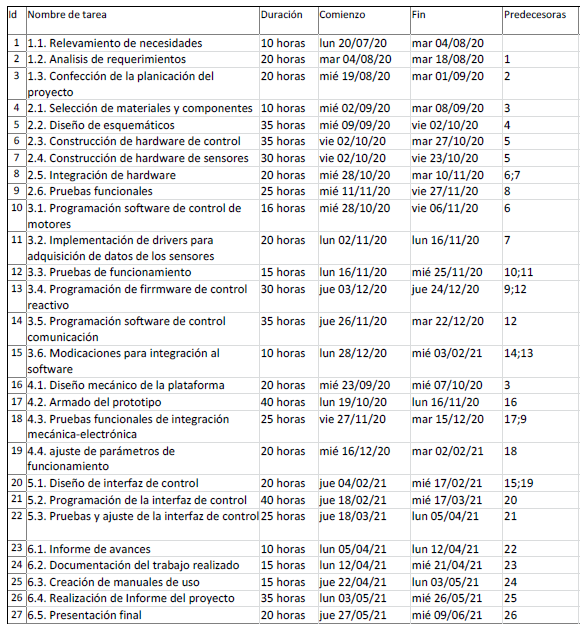
\includegraphics[width=\textwidth]{./Figures/gantttabla.PNG}
%%\caption{Tabla de tareas de Gantt.}
%%\label{fig:gantt1}
%%\end{figure}
%%
%%\begin{figure}[htpb]
%%\centering 
%%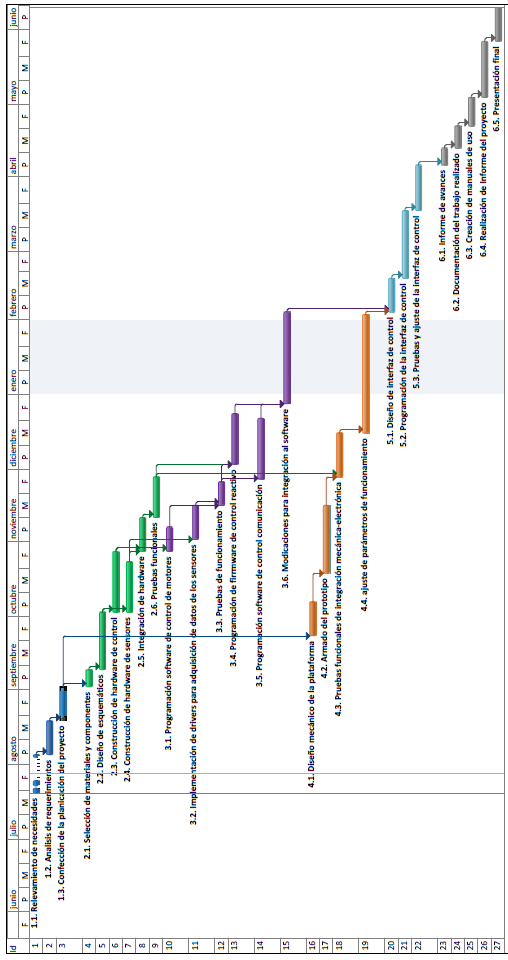
\includegraphics[width=\textwidth]{./Figures/Gantt.PNG}
%%\caption{Diagrama de Gantt.}
%%\label{fig:gantt2}
%%\end{figure}
%%
%%\pagebreak
%%
%%\subsection{Diagrama de Precedencias}
%%Se confeccionó también un diagrama de Precedencias o de Activity on Node (AON), con la finalidad de resaltar las tareas cuyos retrasos podrían resultar críticos para la concreción del trabajo. En rojo se indica el camino crítico, como puede apreciarse en la figura \ref{fig:AoN}
%%
%%\begin{figure}[htpb]
%%\centering 
%%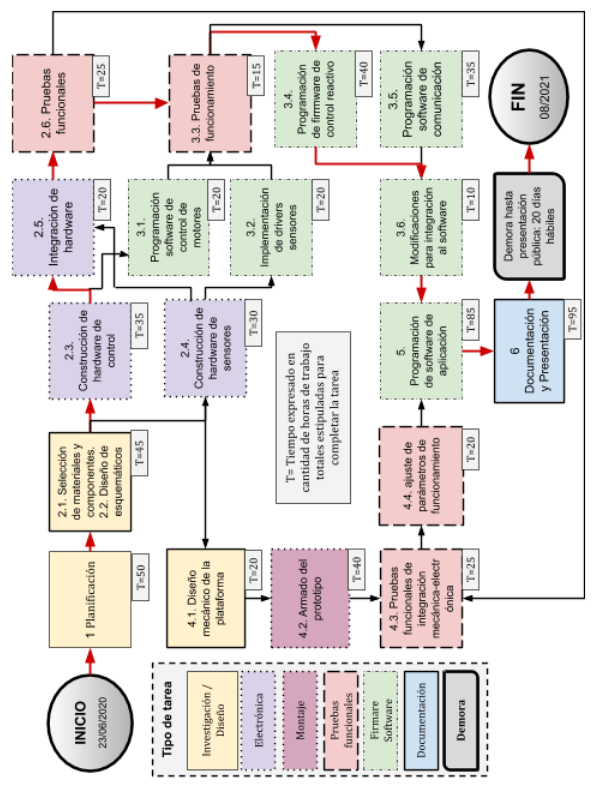
\includegraphics[width=12cm]{./Figures/AoN.png}
%%%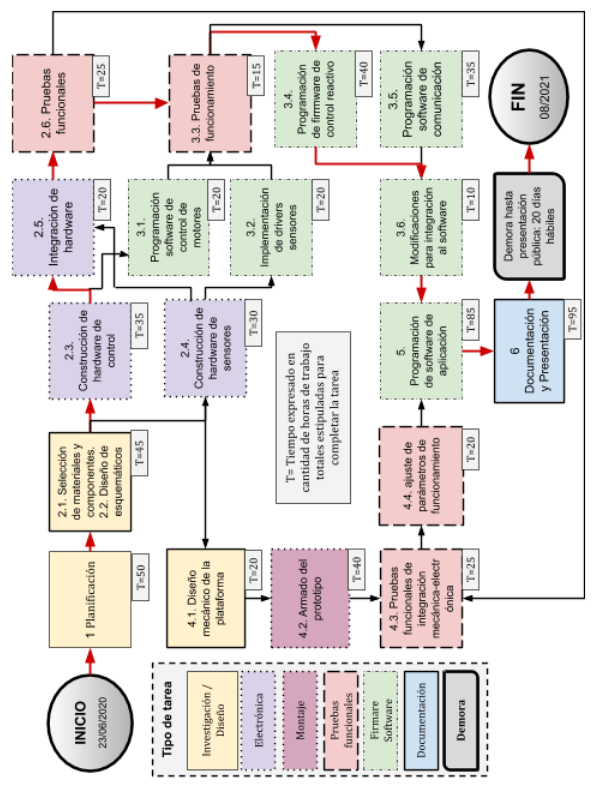
\includegraphics[width=\textwidth]{./Figures/AoN.png}
%%\caption{diagrama de Precedencias o de Activity on Node (AON).}
%%\label{fig:AoN}
%%\end{figure}
%%\pagebreak
%
%\subsubsection{Supuestos iniciales del proyecto}
%
%Para el desarrollo de este trabajo se supuso inicialmente que:
%
%\begin{itemize}
%	\item Se iba a contar con disponibilidad de los laboratorios e instrumental de la  Secretaría de Ciencia, Tecnología e innovación productiva. UTN. Buenos Aires, para cubrir la tarea de desarrollo.
%	\item Se iba a disponer de tiempo durante la jornada laboral para la realización del mismo. 
%	\item Se iba a disponer de todos los componentes y herramientas necesarios.
%\end{itemize}
%
%Estos supuestos, incluidos en la planificación del trabajo, se cumplieron solo en parte, ya que la pandemia por COVID-2019 limitaron el acceso a los laboratorios e instrumental, a la vez que se incrementó el tiempo necesario para las actividades laborales desarrolladas en paralelo al proyecto. 
%
%


